\section{Model Checking}
\subsection{Introduction}
To build our final model, we decided to use an incremental way for the construction, meaning that we started from a Minimum Viable Product that we develop more a little bit more at each step. We  verified each one and, that way, we are assure ourself to have a solid base to continue. Also, that way, we can identify issue more easily.

At the end of the day, we did it in 4 different steps. We will now, explain each step without entering into too much detail except for the final step which will be deeply explained.

\subsubsection{Step 1: Basic Traffic Lights system}
In this first basic step, we created the model in Uppaal of a simple controller sending a pulse every 3 seconds to two cars traffic lights. There is no pedestrians and no buses in this step. \\
Every 3 seconds, the South and North traffic lights switch from green to red while the East and West traffic lights switch, on the opposite, from red to green. \\

Thanks to this basic example, we understood Uppaal basics and notably how it is possible to send messages from one component to an other component thanks to the channel message passing system. \\

In this system, it is possible to check whether our first traffic light is green and the other is red at certain time and vice-versa. Thus we check if we never reach a state where our system is in an impossible and dangerous state where both traffic lights would be green.


\begin{figure}[H]\label{fig:step1}
  \centering
    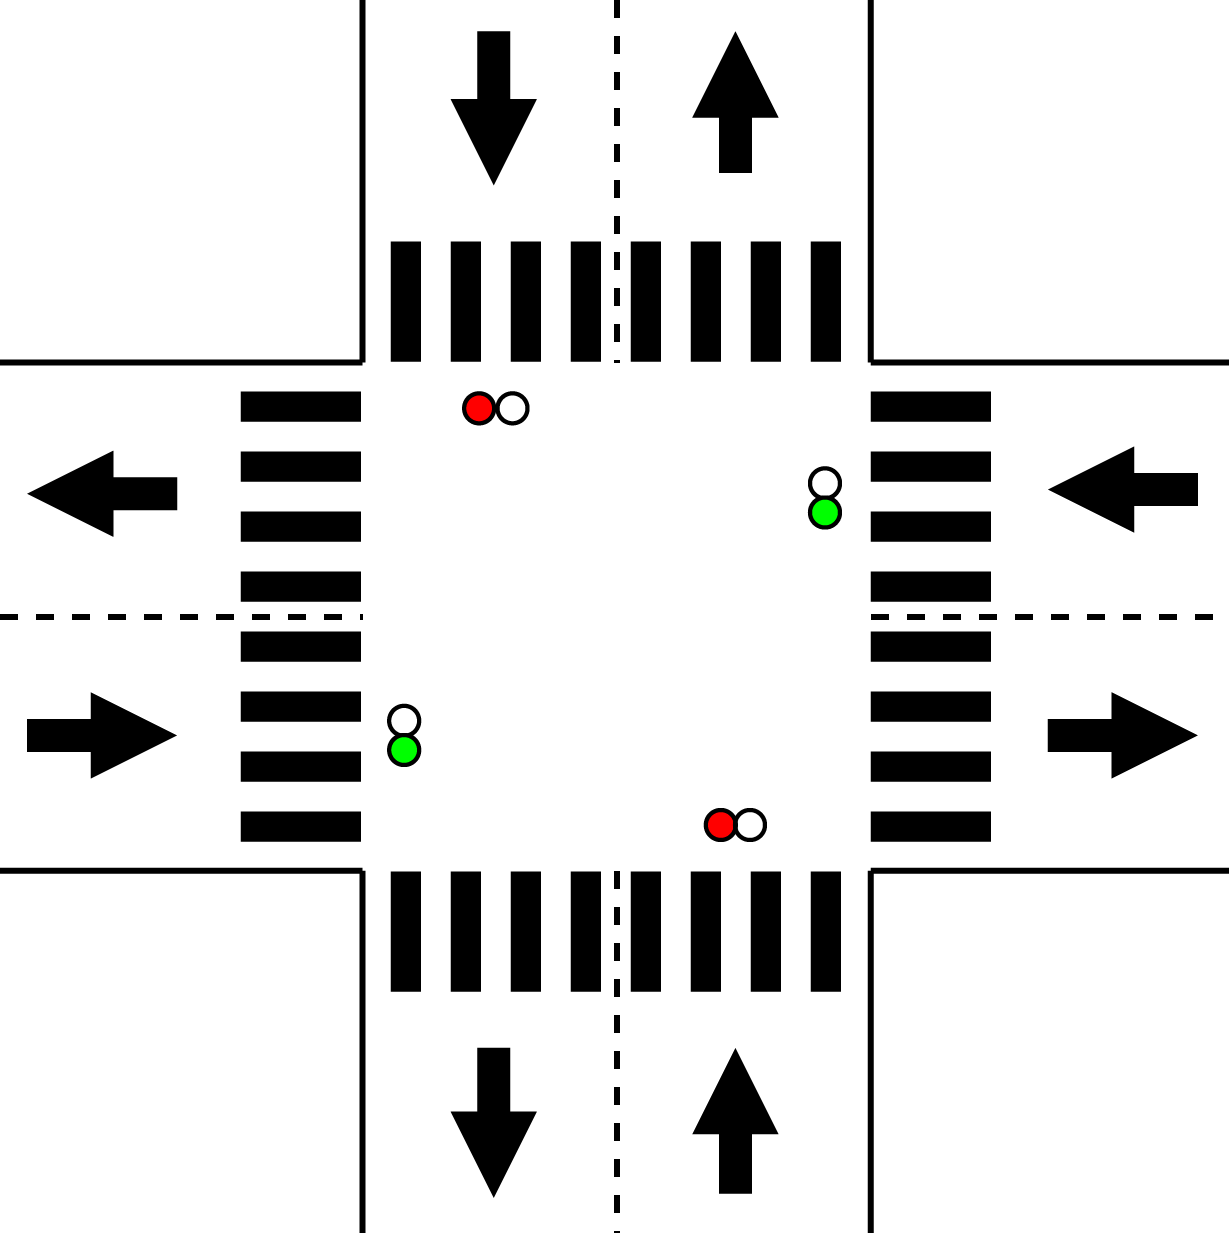
\includegraphics[width=0.5\textwidth]{picture/model/trafficlight_step1_s1.png}
    \caption{Model of the step 1}
\end{figure}

\subsubsection{Step 2: Pedestrians}
In this step, pedestrians were now added and many different things had to be changed to allow accommodate this new change. \\ 

When a pedestrians call was send by the environment, the car's traffic light that was green had to become red and the other car traffic light had to stay red. When those two traffic lights are red, the pedestrians traffic light could be green. Because we also wanted fairness in our system, two assumptions were here created.
\begin{enumerate}
    \item When the pedestrians traffic light is green, we have to remember which car traffic light was previously green. This will be useful for the next assumption.
    \item We wanted fairness between the actors, even if pedestrians have the priority. The problem at the beginning was that starvation could happen if, when the pedestrians lights are green, we always switched to a specific car's traffic light. This would mean that the other car's traffic light would remain red if pedestrians are always calling. We thus added what we called a "delayed" call where, even if the pedestrians are always pressing the button, the two cars lights have to be green at least once before the pedestrians could have their lights green again. This is why the first assumption is useful, we have to remember which car's light was previously green so the cars in the other side of the crossroad don't always have to wait 2 times to be green again. \\
    As an example, if the East-West car's traffic light is green and a pedestrian pressed the button, after the pedestrians lights switch from green to red, the North-South car's traffic light is switched to green so they do not have to wait another time.
\end{enumerate}
In this step, more properties were checked. We for example check if, after a transition, the value of a component always reaches the enquired value. We also check, as for the first one, that certain states can never be reached in our model (all traffic lights are green for example).

\noindent In this step, we also showed thanks to PRISM that our three traffic lights were green with almost the same percentage of time. This can be seen on Figure \ref{fig:prism1}. On this graph, the X-axis represent the average time elapsed between two crosswalk calls while the Y-axis represent the number of times a traffic light is switching to the green state every T (300 in our case) units of time. What we can see is that the more time there is between the pedestrians call, the more our car traffic lights will remain green.

\begin{figure}[H]\label{fig:prism1}
  \centering
    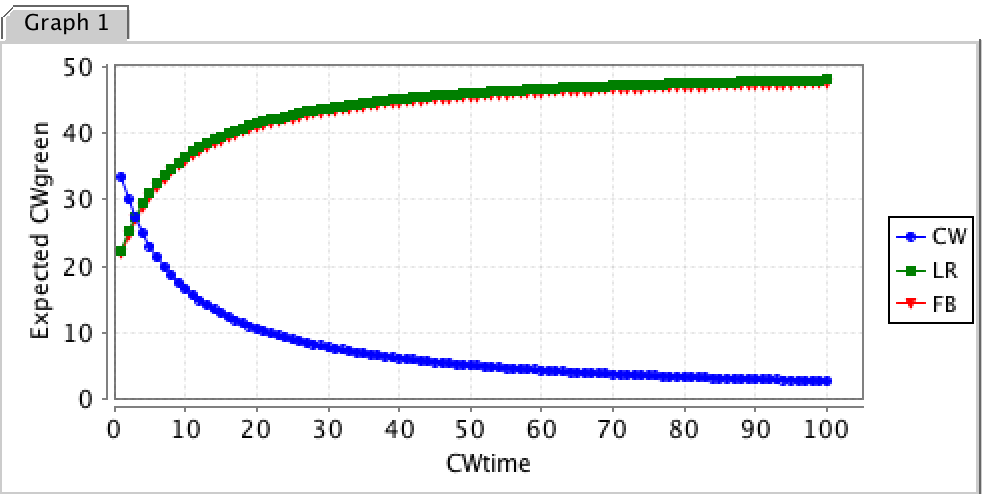
\includegraphics[width=0.5\textwidth]{picture/graphprism.png}
    \caption{Percentage of green lights between the traffic lights}
\end{figure}


\subsubsection{Step 3: Buses}
In this step, we added the buses generated by the environment. The idea here is that the buses have priority on the rest of the traffic. \\
When a bus is generated, the next traffic light that has to be green is the one of the bus. When the bus is crossing, all other lights are red because the bus will go through all the crossroad. The model can be seen as on Figure \ref{fig:step3bus}. \\

\begin{figure}[H]\label{fig:step3bus}
  \centering
    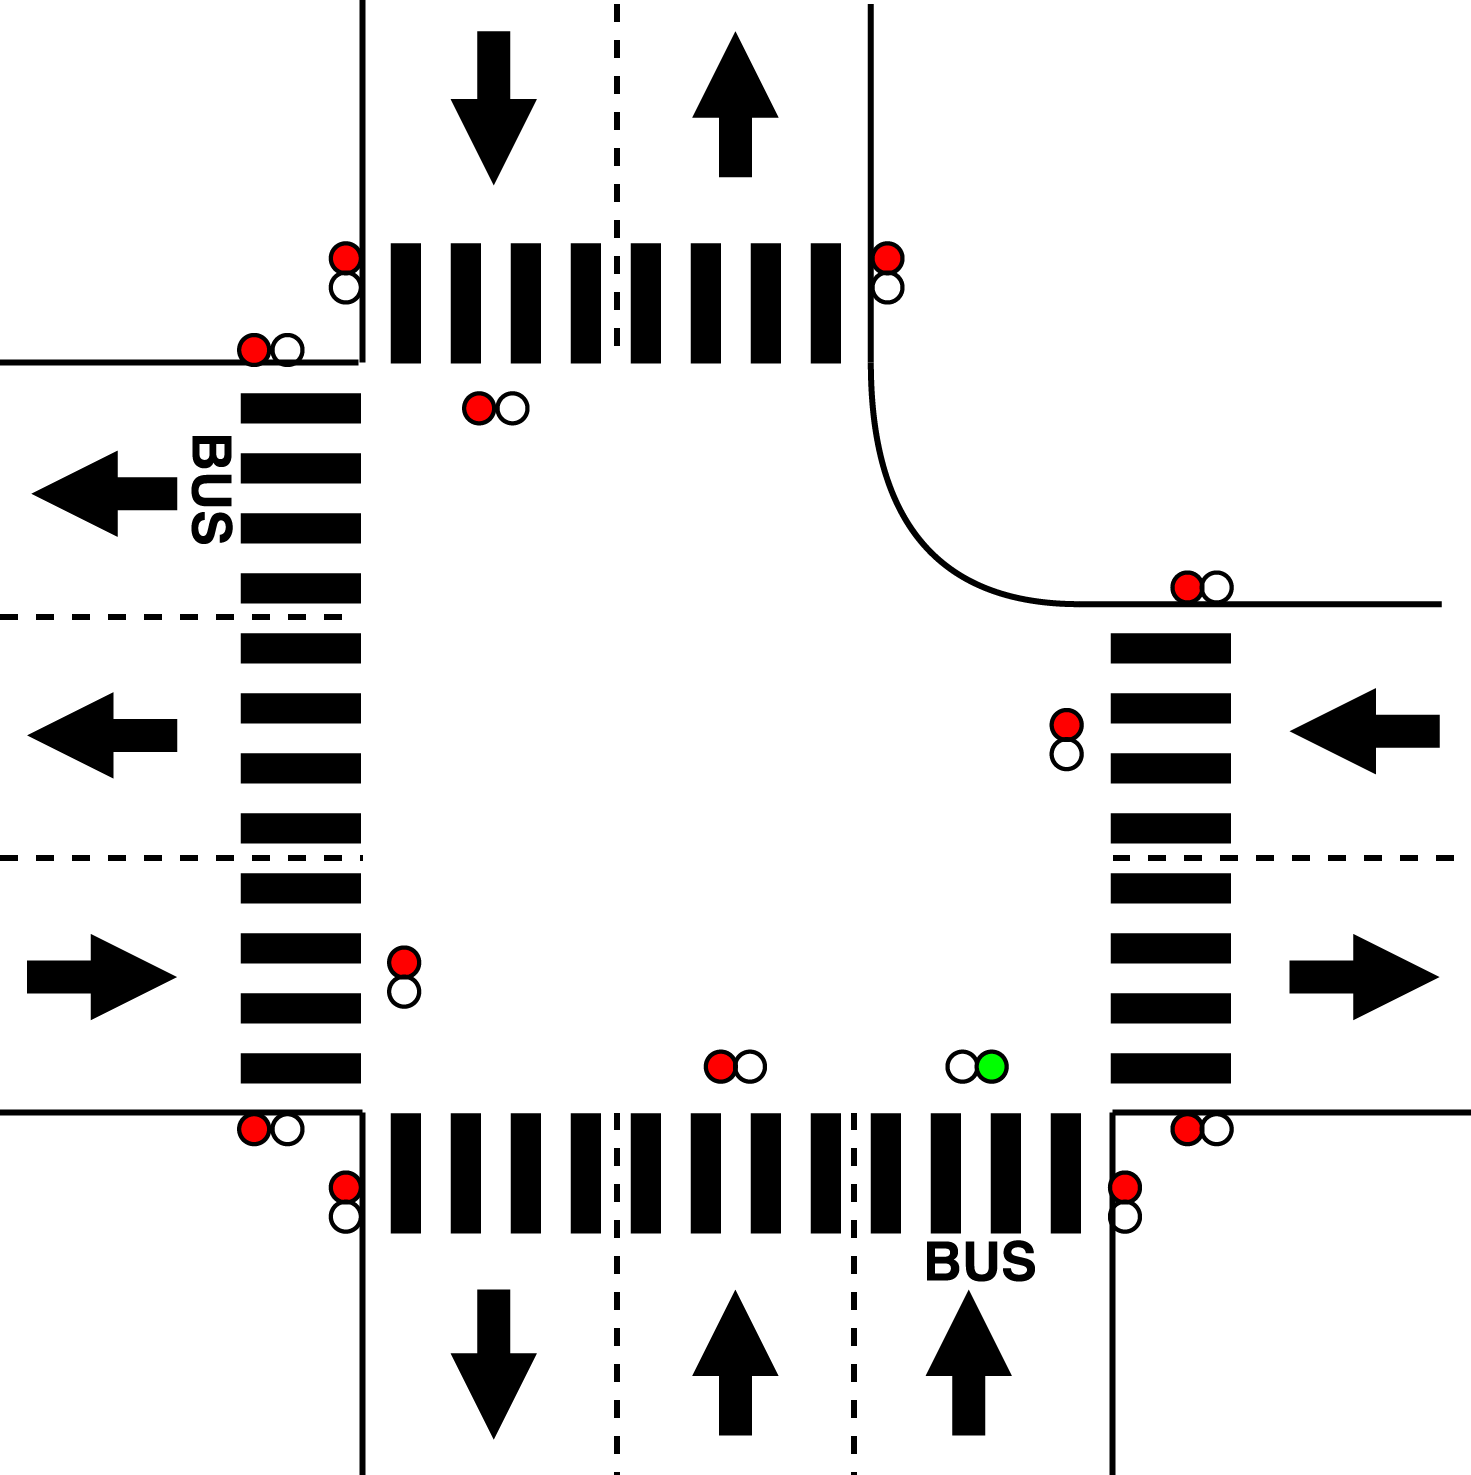
\includegraphics[width=0.5\textwidth]{picture/model/trafficlight_step3_s2.png}
    \caption{Model for the step 3}
\end{figure}

\noindent Even if the pedestrians have called to have the green lights before the bus, if a bus is generated between the call and the pedestrians green light, we will first give the green light for the bus, then the pedestrians, then the cars. This mean that the priority hierarchy is \textit{Buses-Pedestrians-Cars}. \\
This step has also been written in \textbf{PRISM}. Thanks to this complex model, we obtain more specific details about our implementation. We for example could calculate the effect of the time that has elapsed between two buses with as constant the time of a pedestrian call. We also could look at the effect of the time between two pedestrians on the green light of the bus for different time between two buses. \\
Those details can be seen on Figure \ref{fig:cw1}, \ref{fig:cw3} and \ref{fig:busbus}.
\begin{figure}[H]\label{fig:cw1}
  \centering
    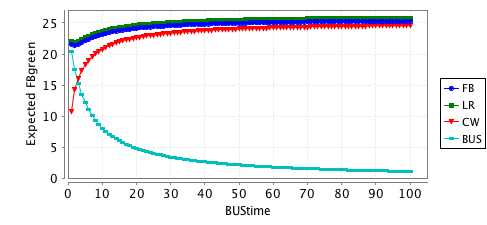
\includegraphics[width=0.5\textwidth]{picture/CWtime1.png}
    \caption{Effect of time that has elapsed between two buses with pedestrian call = 1 unit of time}
\end{figure}

\begin{figure}[H]\label{fig:cw3}
  \centering
    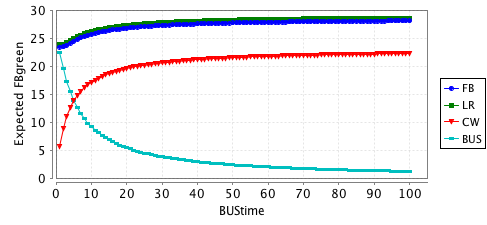
\includegraphics[width=0.5\textwidth]{picture/CWtime3.png}
    \caption{Effect of time that has elapsed between two buses with pedestrian call = 3 units of time}
\end{figure}

\begin{figure}[H]\label{fig:busbus}
  \centering
    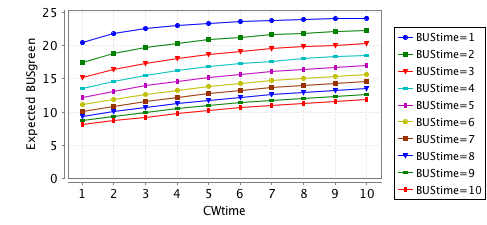
\includegraphics[width=0.5\textwidth]{picture/CWtimeOnBUS.png}
    \caption{Effect of the time between two pedestrians calls on the bus green light}
\end{figure}


\subsubsection{Step 4: Yellow Light}\label{sec:step4}
For this step, we kept the same model done in step 3 but we added a yellow light. This means that, as in the real life, our cars traffic lights will switch from green to yellow to red. \\
This is thus our final model developed in Uppaal TiGa.

\begin{figure}[H]\label{fig:step4}
  \centering
    \includegraphics[width=0.5\textwidth]{picture/model/Trafficlight_step4.png}
    \caption{Model of the step 4}
\end{figure}

\subsection{Timed Automatons}
In order to formally model the system, we use several timed automatons from Uppaal. While some of those automatons are actors in the environment, the others are part of the controller.
The theory tells us that, when the environment is playing, we, humans, cannot decide the action that will be taken. For example, buses and pedestrians arrivals are unpredictable and uncontrollable, so they belong to the environment.
The actors which implement the solution for avoiding crashes belong to the controller. They interact with the environment in order to avoid crashes and thus they aim to find a winning strategy. \\
We will now give the implementations explanations of the environment and controller actors. In the first one, we will take a look at the pedestrians and buses generators while in the second one, we will look at our traffic light system that tries to find a winning situation (no crashes).

\subsubsection{Environment}
\paragraph{Crosswalk} \mbox{}\\
We will here talk about the mechanisms of our crosswalk generator done in our step 4 from Section \ref{sec:step4}. \\
There are several elements that can be seen on Figure 4.1.

\begin{figure}[H]\label{fig:crosswalk}
  \centering
    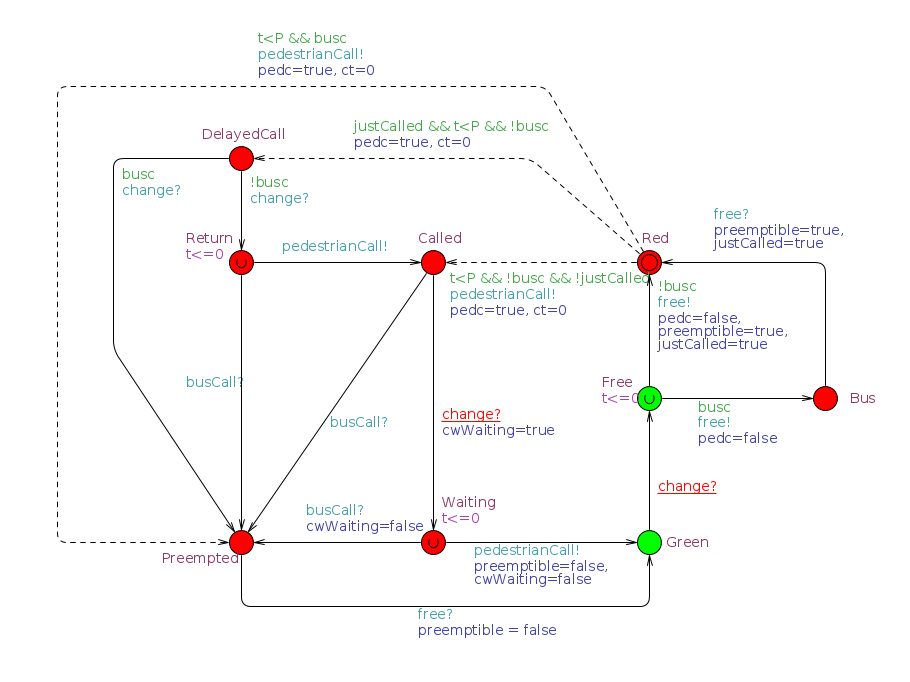
\includegraphics[width=0.9\textwidth]{picture/crosswalk.png}
    \caption{Pedestrians generator}
\end{figure}
\noindent It can first be seen that no orange lights are present here. Indeed, as it was a pedestrians traffic lights in Brussels, there is only the red and green light. We thus decided not to add an orange light for this component. \\
When the environment play, different states can be reaches. Because we said the bus had total priority, different cases can happen. We will first explain the easiest case that can occur. When there is a call for the light to be green, if no buses are generated, we will reach the waiting state. In this state, we will wait for the cars traffic lights to be red, and when it is the case, the pedestrians light can be green. Of course, it is not that simple, since the buses have priority. Indeed, when the fire is in the red state, a transition going to the preempted state ca happen if there is already a bus. When the bus is gone, then the pedestrians lights can be green.\\
Another problem can still happen when the call has been made for the pedestrians light to be green. Indeed, if a bus arrives, it must have the priority on the light. This is why we check, until we allowed the green light, if a bus has been generated. If it is the case, we have to wait for the bus to leave the crossroad and then the pedestrians light can be green. \\
When the green light has to be switched red again, we will first go in a free state where we will check again if another bus has arrived. If an other bus arrives, we let him cross again before releasing the light and then, in any cases (bus or not bus), we go back to the basic red state.
\paragraph{Bus} \mbox{}\\
We will here talk about the mechanisms of our bus generator done in our step 4 from Section \ref{sec:step4}. \\

\begin{figure}[H]\label{fig:bus}
  \centering
    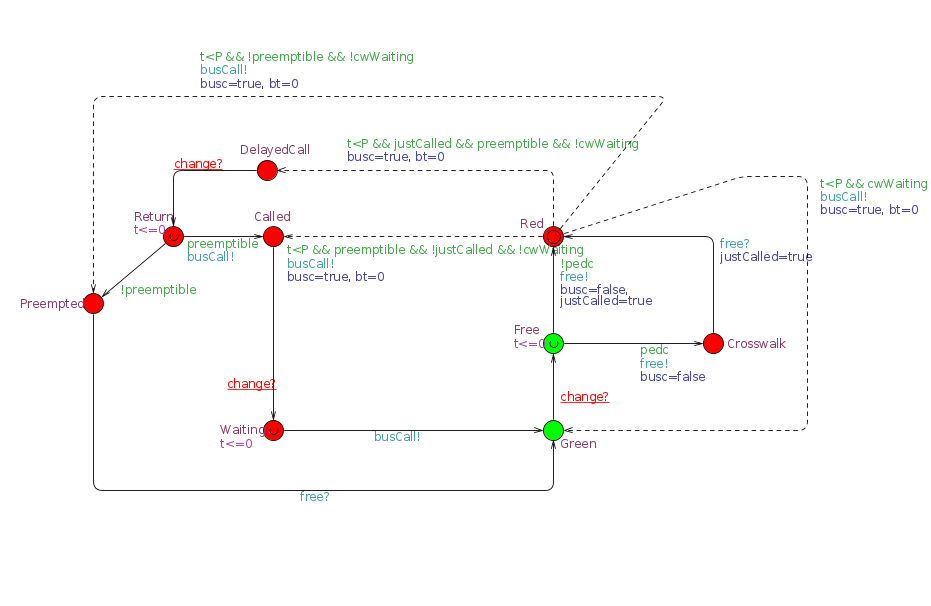
\includegraphics[width=0.9\textwidth]{picture/bus.png}
    \caption{Buses generator}
\end{figure}

\noindent This generator follows the same idea as the pedestrians generator. Since there is nothing that has a higher priority than the bus, the model is easier that the one of the pedestrians. We initially start on a red state. If a bus is called (read generated), we wait for the light that is green on the system to be red. When it is the case, the bus light has to be turn to green. We then also check if pedestrians were generated to allow them to have their light green after. \\

\noindent Those were the two actors controlled by the environment.

\subsubsection{Controller}
\paragraph{Traffic Lights} \mbox{}\\

In this section, we will present the strategy we implemented for the controller to reach a winning strategy. \\

There are two different cars traffic lights. There is the one we called Left-Right, meaning it represents the East-West lights and the Front-Back representing the North-South crossroad. Since the idea is the same, we will just explain the Left-Right one. It just has to be kwown that the initial state for the Left-Right is the red trafic light while for the other one the initial state is the green one. \\

From the red initial state, three different states can be reached:
\begin{enumerate}
  \item If a bus has been called, the traffic light has to remain red so the bus can drive through the crosswalk. We thus reach the \textit{Bus} state.
  \item If pedestrians have pushed the button, we switch to the \textit{Crosswalk} state.
  \item If no buses or pedestrians were generated and the other cars traffic lights is switching to red, we can reach the \textit{Green} state.
\end{enumerate}

\subsection{Tested Propreties}
In this section, we will give and explain the code to formally verify that our system is correct.

\subsubsection{Liveness}
Stifler écrit les propri
\subsubsection{Safety} 
idem